\chapter{Metodologie}\label{teoria}
\pagestyle{fancy}
\fancyhf{}
\fancyhead[OL]{\rightmark}
\cfoot{\thepage}

Come già anticipato, l'approccio più efficace alla risoluzione del problema della classificazione delle immagini consiste nell'impiego delle reti neurali convoluzionali (CNN, \emph{convolutional neural networks}). In questo capitolo saranno introdotti progressivamente i presupposti teorici matematici e informatici su cui si fondano le reti neurali, partendo dalle definizioni preliminari fino a costruire il modello generale di una CNN.



\section{Reti neurali}

TODO: parlare del neurone e dell'idea di replicarlo nella funzione (dopo aver parlato dei classificatori lineari, perché bisogna parlare anche 

\section{Immagini digitali}
Caratterizziamo intuitivamente il concetto di "immagine" dal punto di vista informatico.

Un'\textbf{immagine digitale} è una rappresentazione binaria di un'immagine (in generale a colori) a due dimensioni\footnote{Ci riferiamo in questa sede solo alle immagini di tipo raster, tipiche ad esempio delle fotografie digitali in formato jpg.}; essa può essere definita matematicamente come un tensore $\mathcal{I}\in\R^{h\times w\times c}$, dove $h$ e $w$ sono rispettivamente dette \textbf{altezza} e \textbf{larghezza} dell'immagine, la coppia $(w,h)$ \textbf{risoluzione} mentre $c$ è il numero di \emph{canali di colore}\footnote{Spesso si scrive che $\mathcal{I}$ è un immagine $w\times h\times c$, o più semplicemente $w\times h$ (assumendo $c=3$)}. Nello spazio di colore RGB, ampiamente adoperato, i canali di colore sono rosso (R, Red), verde (G, Green) e blu (B, Blue), quindi $c=3$. In mancanza di diverse indicazioni, ci si riferirà nel seguito allo spazio di colore RGB.

Un \textbf{pixel} $p(i,j)$ è definito come la funzione vettoriale
\[p(i,j)=[r(i,j),g(i,j),b(i,j)]\]
essendo $r,g,b:\{0,\dots,h\}\times\{0,\dots,w\}\to\{0,\dots,255\}$ le funzioni scalari che associano ad ogni posizione bidimensionale $i,j$ dell'immagine un valore intero di \emph{intensità luminosa} compreso tra 0 e 255, uno per ciascuno dei tre canali RGB. Ogni pixel definisce univocamente un colore nello spazio RGB, il quale può rappresentare in tutto $256^{3}$ colori diversi, cioè circa 17 milioni.

\begin{figure}
  \begin{minipage}[b]{0.46\textwidth}
    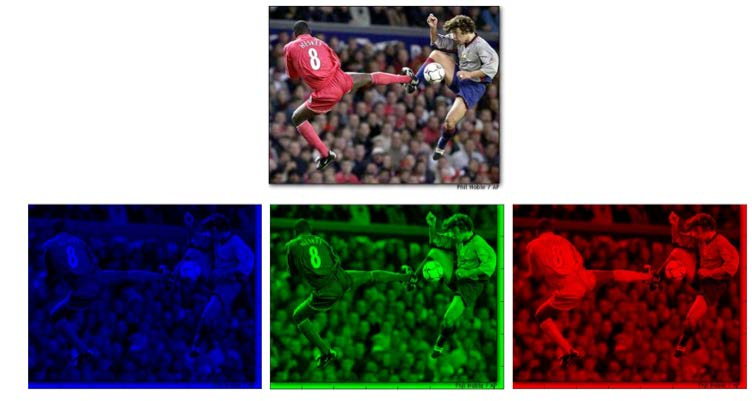
\includegraphics[width=\textwidth]{canali_rgb}
    \caption{Canali RGB di un'immagine}
  \end{minipage}
  \hfill
  \begin{minipage}[b]{0.46\textwidth}
    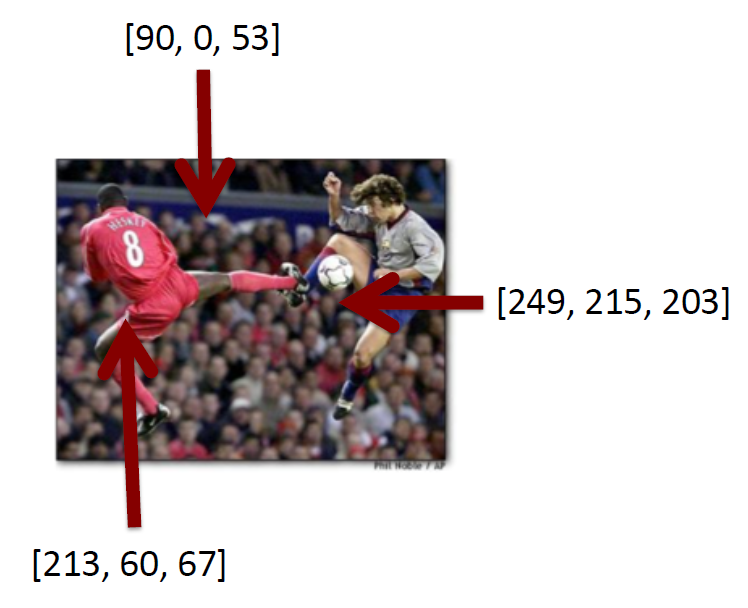
\includegraphics[width=\textwidth]{pixel}
    \caption{Pixel di un'immagine}
  \end{minipage}
\end{figure}

Si può immaginare il tensore immagine $\mathcal{I}$ come una "pila" di tre matrici, una per ogni canale di colore, come mostrato in figura \ref{rappresentazione_tensore}.

\begin{figure}
\centering
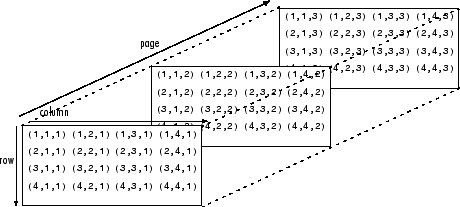
\includegraphics[scale=0.7]{rappresentazione_tensore}
\caption{Rappresentazione grafica di un tensore tridimensionale; in ogni posizione compaiono gli indici del tensore}
\label{rappresentazione_tensore}
\end{figure}

TODO inserire problema dell'object detection pag. 43 Gianvito

\subsection{Supervised Learning}

Il paradigma dell'\textbf{apprendimento supervisionato} (\textit{supervised learning}) si basa sulla creazione di un algoritmo in grado di apprendere una funzione che mappi un input all'output corretto, sulla base di una serie di esempi ideali costituiti da coppie di input e dei relativi output attesi, che gli vengono inizialmente forniti per addestrarlo \cite{Russell2009}.
Un algoritmo di apprendimento supervisionato analizza i dati di addestramento e inferisce una funzione che può essere usata per mappare nuovi input ai corretti output. Ciò richiede all'algoritmo la capacità di trovare una funzione che sappia generalizzare efficacemente dai dati di training, al fine di adattarsi bene a nuovi dati (per poterne mappare correttamente quanti più possibile).\\

Molti problemi pratici, come ad esempio la regressione e la classificazione, possono essere formulati ricorrendo ad una funzione matematica
\[\mathcal{F}:X\to Y\]
che associa ad ogni elemento nello spazio degli input $X$ (dataset) uno ed un solo elemento dello spazio degli output.
Il concetto di funzione implica l'esistenza di un solo elemento di $Y$ a cui ogni elemento di $X$ è correttamente associato. Il problema consiste allora nel cercare una funzione $\mathcal{F}$ in grado di ottenere esattamente tale associazione, per quanti più elementi di $X$ possibile.

È evidente che questo tipo di problemi ben si presta ad essere approcciato con algoritmi di apprendimento supervisionato.

Prima di analizzare in dettaglio il problema di classificazione delle immagini oggetto della presente tesi, è necessario inquadrare il problema partendo da alcune definizioni preliminari.\\

Un \textbf{dataset} X è una generica collezione di $N$ dati
\[X=\{\mathbf{x}^{(1)},\mathbf{x}^{(2)},\dots,\mathbf{x}^{(N)}\}\]
Ogni dato $\mathbf{x}^{(i)}$ è chiamato \textbf{esempio} (o \textbf{data point}).
I data point possono essere anche non omogenei tra loro (cioè avere dimensioni differenti).
Ciascun esempio si può caratterizzare come un vettore $\mathbf{x}^{(i)}\in\R^{D}$, in cui ciascun elemento $x_i$ è detto \textbf{feature} e rappresenta una caratteristica di un oggetto o un evento misurato. $D$ è il numero di feature in ogni esempio, o \textbf{dimensione} dell'esempio.
In caso di esempi omogenei (cioè aventi stessa dimensione $D$) un dataset può essere descritto attraverso una matrice detta \textbf{design matrix}, in cui ogni riga corrisponde ad un particolare esempio e ogni colonna corrisponde ad una precisa feature.
Un dataset di cardinalità $N$ e in cui ogni esempio ha $D$ feature ha quindi una design matrix di dimensione $N\times D$. \\

In un problema di classificazione delle immagini orientato all'\textit{object recognition} (riconoscimento di un oggetto in un immagine), sussiste la seguente caratterizzazione:
\begin{itemize}
\item $X$: un insieme di $N$ immagini digitali
\item $Y$: un insieme di $K$ classi predefinite di oggetti che possono essere individuati all'interno di un'immagine (possono essere dei "descrittori" testuali o, equivalentemente, dei numeri interi)
\end{itemize}
Un elemento di $Y$ è solitamente chiamato \textbf{etichetta} o \textbf{categoria} (in inglese \textbf{label} o \textbf{class}); si dice quindi che ogni immagine $\mathbf{x}^{(i)}\in X$ può essere \textit{descritta da un'etichetta} (o \textit{associata ad una categoria}) $\mathbf{y}^{(i)}\in Y$ tramite una funzione di associazione $f$.\footnote{Teoricamente una stessa immagine potrebbe essere descritta da più di un'etichetta o addirittura da nessuna, coerentemente col fatto che in essa potrebbero essere presenti più oggetti o nessun oggetto tra quelli previsti in $Y$. Tuttavia nella presente tesi questa ambiguità non può sussistere: la classificazione riduce qualsiasi immagine ad una di due categorie mutualmente esclusive e di cui almeno una deve essere ammessa, cioè la presenza o meno di una pinna nell'immagine.}\\
Nella pratica, TODO f non può essere trovata esattamente. (vd gianvito)

TODO: scrivere ora o in un paragrafo a parte i tipi di dato per gestire le immagini messi a disposizione da matlab.


\section{Classificatore lineare}
Il classificatore lineare è una tra le più semplici funzioni di classificazione.\footnote{La fonte principale per gli argomenti trattati in questo paragrafo è \cite{cs231n}}
Ipotizziamo di avere un insieme di $N$ immagini $\mathbf{x}^{(i)}$ (\textit{data points}), ciascuna con risoluzione fissa $w\times h$ e in formato RGB ($c=3$), e un insieme di $K$ distinte categorie di oggetti  (\textit{labels}). Un \textbf{classificatore lineare} è definito dalla funzione
\begin{equation} \label{eq_class_lin}
f(\mathbf{x}^{(i)};\mathbf{W},\mathbf{b})=\mathbf{W}\mathbf{x}^{(i)}+\mathbf{b}
\end{equation}
In questa espressione stiamo assumendo che $\mathbf{x}^{(i)}$ sia un vettore colonna di dimensione $D=hwc$ ottenuto incolonnando una ad una le righe dell'$i$-esima immagine di tutti e tre i canali di colore, $\mathbf{W}$ una matrice detta \textbf{matrice dei pesi} (\textit{weights matrix}) di dimensione $K\times D$ e $\mathbf{b}$ un vettore colonna detto \textbf{vettore dei bias} (\textit{bias vector}) di dimensione $K$. I pesi e i bias sono parametri della funzione $f$.

Ogni riga $j$-esima di $W$ e il relativo $j$-esimo valore di $\mathbf{b}$ serve a calcolare la combinazione (lineare a meno del bias) $\mathbf{w}_j\cdot \mathbf{x}^{(i)}+b_j$. Ognuna delle $K$ combinazioni calcolate è un numero reale che si può interpretare come un "punteggio" registrato dall'$i$-esima immagine in ogni classe di oggetti in $Y$ (\textit{class score}): l'$i$-esima immagine è classificata con l'etichetta $\mathbf{y}_j\in Y$ se l'elemento $j$-esimo del vettore output $f(\mathbf{x}^{(i)};\mathbf{W},\mathbf{b})$ è il massimo del medesimo vettore.\\

L'esempio in figura \ref{class_lin} mostra la classificazione di un'immagine di un gatto con $\abs{Y}=3$ classi (\textit{gatto}, \textit{cane}, \textit{barca}). Per semplicità, l'immagine input è ipotizzata $2\times 2$ e composta da un unico canale di colore ($c=1$) (quindi $\mathbf{x}$, scritta come vettore colonna, è $4\times 1$).

\begin{figure}[h]
\centering
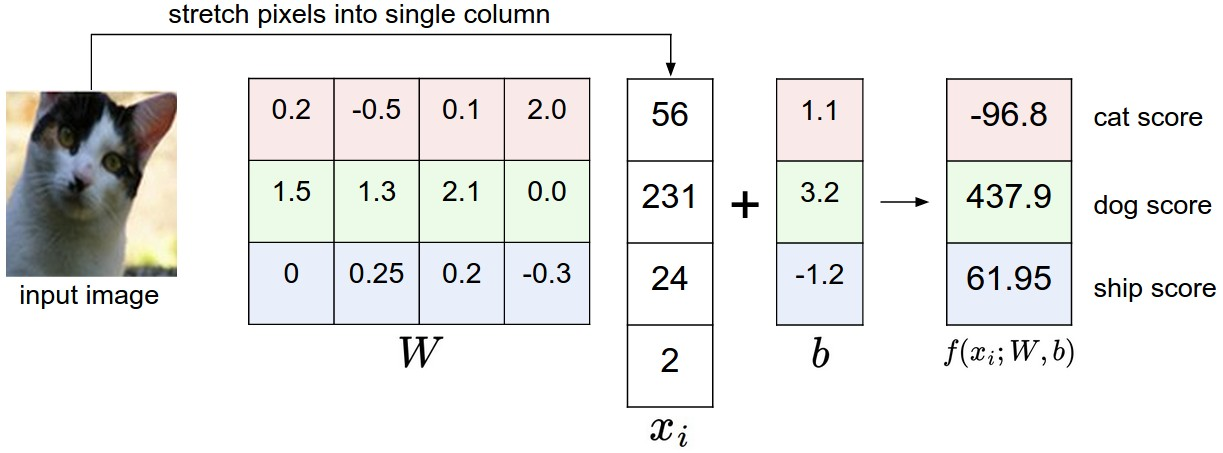
\includegraphics[width=\textwidth ,keepaspectratio]{classificatore_lineare}
\caption{Mappatura di un'immagine ai punteggi di ogni classe mediante un classificatore lineare. Si noti che i pesi di $\mathbf{W}$ non costituiscono un buon set di parametri: il punteggio assegnato alla classe "cane" (sbagliata) è alto e quello totalizzato dalla classe "gatto" (corretta) è basso. Il classificatore "è convinto" di aver classificato l'immagine di un cane.}
\label{class_lin}
\end{figure}

\subsection*{Interpretare un classificatore lineare}

Poiché le immagini possono essere memorizzate come vettori colonna $hwc$-dimensionali, si possono immaginare le immagini di un dataset come dei punti nello spazio $\R^{hwc}$. Di conseguenza, il dataset può essere pensato come una collezione di punti multidimensionali. Ovviamente non possiamo visualizzare spazi con più dimensioni di $\R^{3}$, ma se immaginiamo di "comprimere" tutte le $hwc$ dimensioni in sole due dimensioni otteniamo una visualizzazione del tipo in figura \ref{visual_class_lin}.

\begin{figure}[h]
\centering
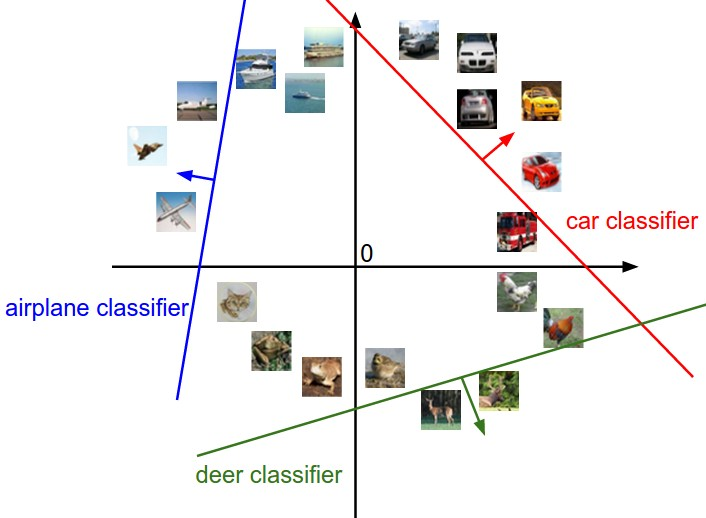
\includegraphics[width=\textwidth ,keepaspectratio]{visualizz_class_lin}
\caption{Visualizzazione di tre righe di un classificatore lineare, una per ciascuna delle classi "aereo", "auto", "cervo".}
\label{visual_class_lin}
\end{figure}

Le rette in figura devono in realtà essere pensate come degli iperpiani $(hwc-1)$-dimensionali, associati a ciascuna classe di $Y$ (cioè a ciascuna riga di $\mathbf{W}$ e $\mathbf{b}$), e il piano come lo spazio $\R^{hwc}$. Sussistono le seguenti interpretazioni geometriche:
\begin{itemize}
\item Le immagini sono dei punti nel piano. Ogni retta è il luogo dei punti che totalizzano un punteggio nullo per la classe associata a quella retta (la classe è scritta in figura accanto ad ogni retta). La freccia nella figura indica la direzione seguendo la quale i punti del piano aumentano (linearmente) il punteggio realizzato per quella classe.
\item Modificare i pesi di $\mathbf{W}$ significa regolare l'inclinazione delle rette (cioè ruotarle rispetto al punto di intercetta).
\item Modificare i bias di $\mathbf{b}$ significa regolare l'intercetta delle rette (cioè traslarle verticalmente).
\end{itemize}

Un altro modo di interpretare i pesi $\mathbf{W}$ può essere quello di far corrispondere ogni riga di $\mathbf{W}$ a un \textbf{prototipo} (in inglese \textbf{template}) per una delle classi. In questa interpretazione, il punteggio realizzato per ogni classe da un'immagine è ottenuto attraverso l'operazione di prodotto matriciale tra il prototipo della classe $j$ ($\mathbf{w}_j$) e l'immagine da classificare ($\mathbf{x}^{(i)}$).
Usando la terminologia introdotta, possiamo affermare che ciò che sta facendo il classificatore lineare è un'operazione di \textit{template matching}, dove i \textit{templates} sono oggetto di apprendimento da parte del classificatore\footnote{Si introdurranno gli algoritmi di apprendimento (supervisionato) nel capitolo \ref{TODO}.}.

Ad esempio, analizziamo il dataset \textit{CIFAR-10} \cite{cifar10}. Esso contiene immagini $32\times 32$ ciascuna appartenente ad una di 10 classi. Visualizzando\footnote{TODO Per i dettagli su come "visualizzare" i pesi si veda \url{https://it.mathworks.com/help/deeplearning/examples/visualize-activations-of-a-convolutional-neural-network.html}.} i pesi (e quindi i 10 templates) di un classificatore lineare addestrato su CIFAR-10 si ottengono i risultati in figura seguente:

\begin{figure}[h]
\centering
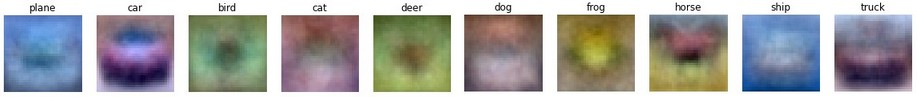
\includegraphics[width=\textwidth ,keepaspectratio]{templates}
\caption{Visualizzazione dei templates di un classificatore addestrato sul dataset CIFAR-10}
\label{templates}
\end{figure}

Si possono fare alcune interessanti osservazioni.

Ad esempio, il prototipo della classe "barca" è composto da molti pixel blu disposti perlopiù lungo i margini, come ci si potrebbe aspettare dal momento che molte immagini di barche in CIFAR-10 raffigurano queste in mare aperto. Questo template allora assegnerà un punteggio alto quando l'immagine che si vuole classificare (cioè \textit{raffrontare al template}) è una barca in mare aperto. In altre parole, un'immagine realizzerà un punteggio tanto più alto in una certa classe quanto più essa è \textit{simile} al template che il classificatore lineare \textit{ha imparato} per quella classe.

Il prototipo per la classe "cavallo" sembra essere l'immagine di un cavallo a due teste; similmente, quello per la classe "auto" sembra una miscela di rappresentazioni di un'auto vista da più direzioni diverse. Ciò è coerente col fatto che il classificatore lineare è stato addestrato su immagini di cavalli visti rispetto a entrambi i profili e su immagini
di auto raffigurate in tante direzioni diverse. Inoltre, il template per l'auto sembra rappresentare un'auto di colore rosso: evidentemente in CIFAR-10 la maggior parte delle automobili rappresentate sono di quel colore.\\

Come si vedrà nel seguito, questa operazione di \textit{template matching} presenta una forte analogia con il funzionamento di un \textit{Fully Connected Layer} di una rete neurale convoluzionale.

\subsection*{Bias trick}
Concludiamo questo capitolo menzionando un "trucco" matematico molto utilizzato per rappresentare $\mathbf{W}$ e $\mathbf{b}$ come un'unica matrice, semplificando la notazione \ref{eq_class_lin}.
Possiamo aggiungere il vettore dei bias in coda alla matrice dei pesi e aggiungere un "1" in coda al vettore che rappresenta l'immagine. In questo modo, il classificatore lineare è rappresentato dalla funzione di associazione
\begin{equation} \label{eq_bias_trick}
f(\mathbf{x}^{(i)};\mathbf{W})=\mathbf{W}\mathbf{x}^{(i)}
\end{equation}

In questa maniera, $f$ calcola solo combinazioni lineari (un singolo prodotto matriciale), poiché il vettore dei bias è stato eliminato.
Tale utile passaggio, noto come \textit{bias trick}, è visualizzato nella seguente figura

\begin{figure}[h]
\centering
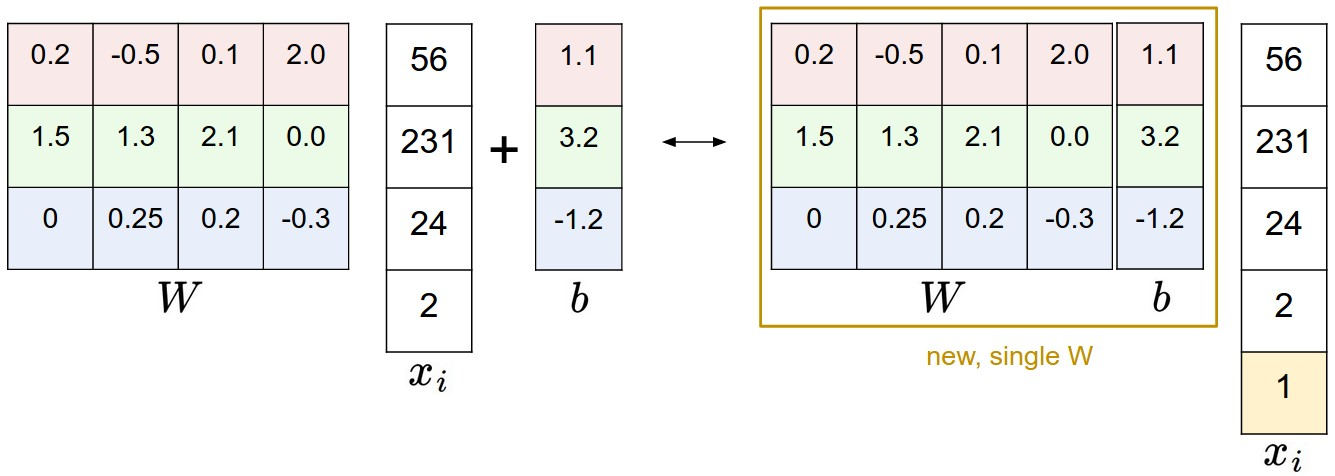
\includegraphics[width=\textwidth ,keepaspectratio]{bias_trick}
\caption{Bias trick}
\label{bias_trick}
\end{figure}

TODO: loss functions.

TODO: valutazione delle prestazioni di una rete neurale (matrice di confusione)